\section{Mesure implicite} % (fold)
\label{sec:supervision_active_&_passive}

\begin{frame}{Introduction}

\begin{block}{Supervision}
  \begin{itemize}
    \item Collecte de données
    \item Interprétation des données
    \item Prise de décisions
  \end{itemize}
\end{block}

\begin{alertblock}{Objectifs}
  \begin{itemize}
    \item Diagnostiquer les pannes
    \item Anticiper les problèmes
    \item Mesure le système
  \end{itemize}
\end{alertblock}

  \pnote{
    - Nombreux produits disponibles dans l'Industrie
    - Nécessité pour prendre des décisions sur l'état d'un système
  }

\end{frame}

\begin{frame}{État de l'art}
  \begin{block}{Supervision active}
    \begin{itemize}
      \item Envoi de statut périodique de la part des nœuds (``health report'', SNMP)
      \item Sondes tierces
    \end{itemize}
  \end{block}

  \begin{block}{Limitations}
    \begin{itemize}
      \item Oblige les nœuds à avoir un agent actif spécifique
      \item Pour les sondes tierces, elles ont également besoin d’être sondées
      \item Trafic supplémentaire
    \end{itemize}
  \end{block}

  \pnote{
    Avec SNMP tu peux avoir un modèle client serveur mais aussi des traps pour l'envoi de notifications.
  }
  \pnote{
    Par contre le protocole SNMP peut être lourd à implémenter (support des MIB Management Information Base pas forcément exhaustif, plusieurs versions du protocole (3 version), dans la troisième qui est sécurisée: pas de négociation de chiffrement =>Doit connaître à l'avance le chiffreur utilisé)
  }
  \pnote{
    - Des nœuds venant de deux vendeurs différents vont pas forcément être supervisés de la même manière
  }
  \pnote{
    - Pas toujours possible de déployer un agent actif sur chaque nœud (plateforme fermée, manque de ressources)
  }

\end{frame}

\begin{frame}\frametitle{Problématiques et contributions}

  \begin{block}{Buts}
    \begin{itemize}
      \item Produire une estimation de l'utilisation de la radio
      \item La radio est la principale consommatrice d'énergie
      \item Avoir une vue du trafic réseau et identifier les points chauds
    \end{itemize}
  \end{block}

  \begin{block}{Solutions classiques de supervision}
    \begin{itemize}
      \item Supervision active parfois indisponible
      \item Consommatrice d'énergie \& inefficace avec des nœuds souvent en sommeil
    \end{itemize}
  \end{block}

  \begin{alertblock}{Contribution}
    \begin{itemize}
      \item Supervision passive de la consommation énergétique à la passerelle
      \item Utilisation de la topologie réseau pour inférer le coût des retransmissions
      \item Correction de cette estimation avec de la supervision active quand c'est possible
    \end{itemize}
  \end{alertblock}

\end{frame}

\begin{frame}{Mesures implicites}
  \begin{block}{Définitions}
    \begin{itemize}
      \item Une mesure active nécessite un envoi de paquets dédiés à cette mesure.
      \item Une mesure passive ne dépend que des paquets qui seraient envoyés de toute façon, même si la mesure n'avait pas lieu.
    \end{itemize}
  \end{block}
  \begin{block}{Propriétés des mesures passives}
    \begin{itemize}
      \item Elles sont fondées sur l'observation de paquets non modifiés et non perturbés.
      \item Une méthode passive ne laisse aucune trace sur le réseau.
      \item Elles ne sont donc utiles que s'il existe déjà des paquets intéressants.
      \item Exemple: sFlow, netflow, IPFIX.
    \end{itemize}

  \end{block}

  \pnote{
    - Le passif n'en créent pas et n'en modifient pas (rfc 7799)
  }
\end{frame}

\begin{frame}{Architecture de mesure implicite}
  \begin{figure}
    \centering
    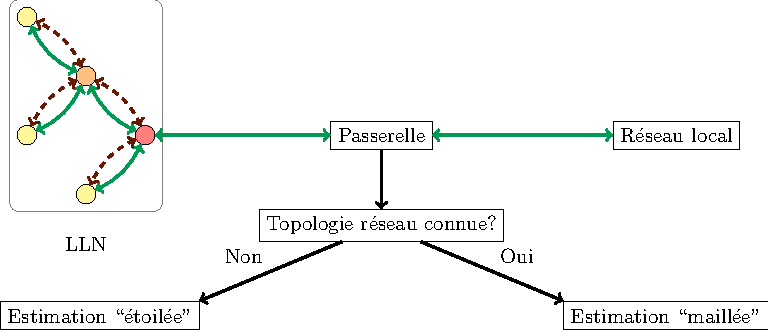
\includegraphics[width=\textwidth]{figures/schema_supervision_slides.pdf}
  \end{figure}
  \begin{block}{Modèle}
    \begin{itemize}
      \item Modélisation de la couche MAC
    \end{itemize}
  \end{block}
\end{frame}

\begin{frame}{Modélisation des transmissions}
  \begin{figure}
      \begin{tikzpicture}
  \tikzstyle{router}=[circle, draw, fill=orange!50,text=black]
  \tikzstyle{child}=[circle, draw, fill=yellow!50,text=black]
  \tikzstyle{root}=[circle, draw, fill=red!50,text=black]
  \tikzstyle{source}=[circle, draw, fill=green!50,text=black]
  \tikzstyle{idle}=[circle, draw, text=black]

  \node[idle] (00) at (0,0) {I};
  \node[child] (10) at (1,0) {O};
  \node[router] (20) at (2,0) {R};
  \node[router] (30) at (3,0) {R};
  \node[source] (40) at (4,0) {A};

  \node[idle] (01) at (0,1) {I};
  \node[idle] (11) at (1,1) {I};
  \node[root] (21) at (2,1) {B};
  \node[child] (31) at (3,1) {O};
  \node[child] (41) at (4,1) {O};

  \path
  % Radio link
  (00.east) edge[dashed] (10.west)
  (10.east) edge[dashed] (20.west)
  (20.east) edge[dashed] (30.west)
  (30.east) edge[dashed] (40.west)

  (01.east) edge[dashed] (11.west)
  (11.east) edge[dashed] (21.west)
  (21.east) edge[dashed] (31.west)
  (31.east) edge[dashed] (41.west)

  (00.north) edge[dashed] (01.south)
  (10.north) edge[dashed] (11.south)
  (20.north) edge[dashed] (21.south)
  (30.north) edge[dashed] (31.south)
  (40.north) edge[dashed] (41.south)

  % Route link
  (40.west) edge[->, very thick] (30.east)
  (30.west) edge[->, very thick] (20.east)
  (20.north) edge[->, very thick] (21.south)
  ;

  \end{tikzpicture}
  \end{figure}
  \begin{block}{Estimation ``étoilée'' (Sans connaissance de la topologie)}
    \begin{itemize}
      \item Source et destination
      \item Aucune connaissance de la topologie
    \end{itemize}
  \end{block}
  \begin{block}{Estimation ``maillée'' (Avec connaissance de la topologie)}
    \begin{itemize}
      \item Source et destination
      \item Pris en compte du relayage dans la mise à jour des compteurs
    \end{itemize}
  \end{block}
\end{frame}

\DeclarePairedDelimiter{\ceil}{\lceil}{\rceil}

\begin{frame}{\ieee{} \& ContikiMAC}
  \begin{block}{\ieee{}}
    $T_p = \frac{\mathcal{L}(f)}{R} \ceil[\Big]{\frac{\mathcal{L}(p)}{L}}$
  \end{block}

  \begin{figure}[ht]
    \centering
    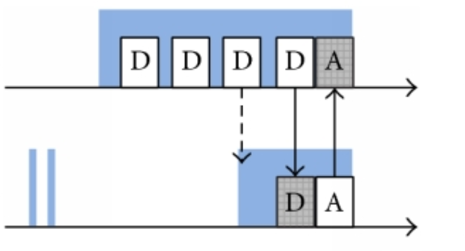
\includegraphics[width=.5\textwidth]{figures/contikimac.png}
    \caption{Schéma d'endormissement dans ContikiMAC}
  \end{figure}

  \begin{block}{Facteur de ``strobing''}
    $N_{\textrm{receiver}} = 1.5$
  \end{block}

  \pnote{
    - En blue: La fenetre de réception
  }
  \pnote{
    - blanc: Trame de données/ack transmises mais non reçue
  }
  \pnote{
    - noir: Trame de données/ack transmis et reçue
  }
  \pnote{
    $T_\detect$ est le temps que le transmetteur va passer en écoute juste après une tentative de transmission pour détecter son éventuel succès par un acquittement d'un récepteur juste après l'envoi d'une trame de donnée.
  }
  \pnote{
    ti: the interval between each packet transmission. (0.4 ms)
  }
  \pnote{
    tr: the time required for a stable RSSI, needed for a stable CCA indication.
  }
  \pnote{
    tc: the interval between each CCA.
  }
  \pnote{
    ta: the time between receiving a packet and sending the acknowledgment packet.
  }
  \pnote{
    td: the time required for successfully detecting an acknowledgment from the receiver. (0.16 ms)
  }
  \pnote{
    ts, the transmission time of the shortest packet, must be larger than tr + tc + tr (0.884 ms)
  }
\end{frame}

\begin{frame}{Strobing moyen $N_{\textrm{sender}}$}
  \begin{block}{Conditions expérimentales}
    \begin{itemize}
      \item Topologie binaire
      \item Rime stack (\ieee{} et ContikiMAC)
    \end{itemize}
  \end{block}
  \begin{figure}
    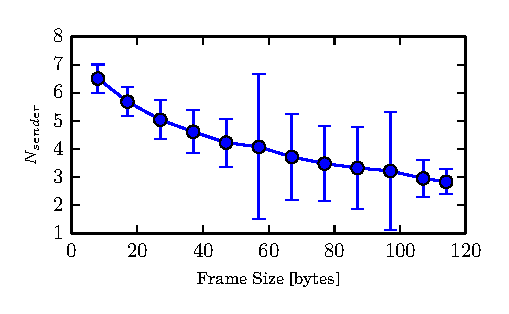
\includegraphics[width=.8\textwidth]{figures/average_strobbing.pdf}
  \end{figure}
  \pnote{
    - Une trame longue est détectée plus facilement car elle a plus de chance de tomber entre deux réveils d'un destinataire
  }
\end{frame}

\begin{frame}{Validation expérimentale}
  \begin{block}{Hypothèses}
    \begin{itemize}
      \item Contiki/COOJA/Powertracker
      \item 200 secondes
      \item 1 paquet/s (69 octets sur le médium)
      \item $N_{\textrm{sender}} = 3.76$
    \end{itemize}
  \end{block}
  \begin{figure}
    \centering
      \begin{tikzpicture}

  % définition des styles
  \tikzstyle{child}=[circle, draw, fill=yellow!50,text=black]
  \tikzstyle{router}=[circle, draw, fill=orange!50,text=black]
  \tikzstyle{root}=[circle, draw, fill=red!50,text=black]

  % Réseau contraint
  \node[root] (root) {G};
  \node[router, left=of root] (1) {1};
  \node[router, left=of 1] (2) {2};
  \node[router, left=of 2] (3)  {3};
  \node[router, left=of 3] (4) {4};
  \node[router, left=of 4] (5) {5};
  \node[child, left=of 5] (6) {6};

\path

  (6.east) edge[->, thin] (5.west)
  (5.east) edge[->, thin] (4.west)
  (4.east) edge[->, semithick] (3.west)
  (3.east) edge[->, thick] (2.west)
  (2.east) edge[->, very thick] (1.west)
  (1.east) edge[->, ultra thick] (root.west)
  ;

  \end{tikzpicture}
  \end{figure}
  \pnote{
    Choix de la chaine: Interprétation facile des résultats de topologie par rapport à une topologie quelconque.
  }
\end{frame}

\begin{frame}{Validation expérimentale}
    \begin{figure}
    \centering
    \subfloat[Répartition par profondeur]{
        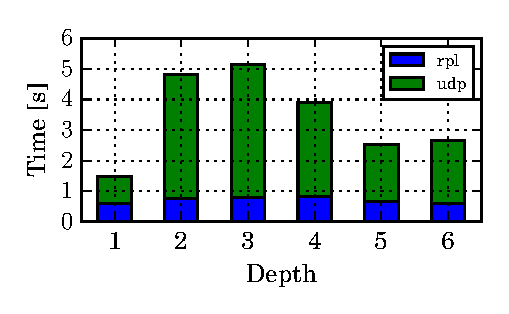
\includegraphics[width=0.5\textwidth]{figures/protocol_repartition_depth.pdf}}
    \subfloat[Évolution au cours du temps]{
        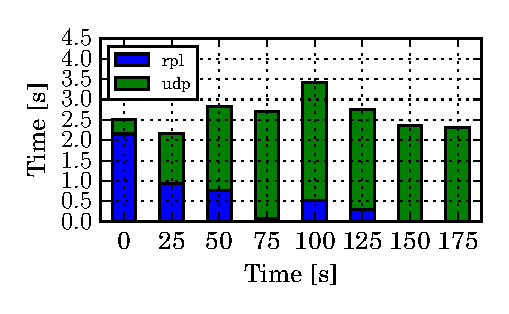
\includegraphics[width=0.5\textwidth]{figures/repartition_protocol.pdf}}
    \caption{Analyse des protocoles}
    \end{figure}
\end{frame}

\begin{frame}{Validation expérimentale}
    \begin{figure}
    \centering
    \subfloat[Packet Delivery Ratio (PDR)]{
        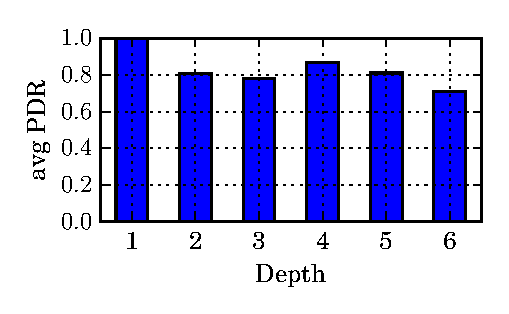
\includegraphics[width=0.5\textwidth]{figures/pdr_depth.pdf}}
    \subfloat[Strobbing par profondeur]{
        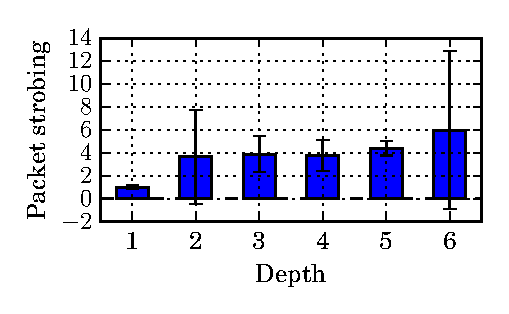
\includegraphics[width=0.5\textwidth]{figures/strobes_depth.pdf}}
    \caption{Impact de la profondeur}
    \end{figure}
\end{frame}

\begin{frame}{Validation expérimentale}
    \begin{block}{Précision}
      $$\delta = \frac{\widehat{X}}{X}$$
    \end{block}

    \begin{figure}
    \centering
    \subfloat[Estimation ``étoilée'' \label{fig:1}]{
        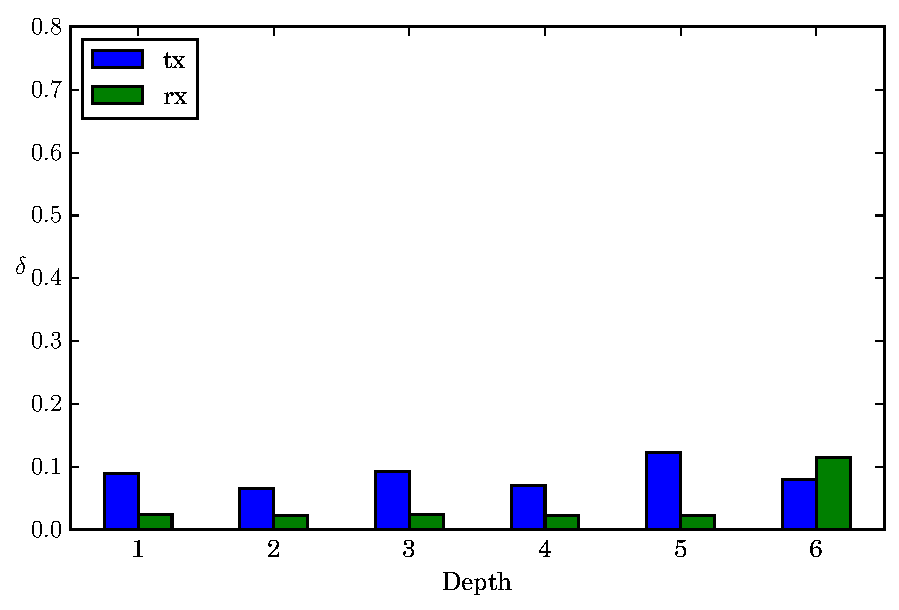
\includegraphics[width=0.5\textwidth]{figures/global_noinfo.pdf}}
    \subfloat[Estimation ``maillée'' \label{fig:2}]{
        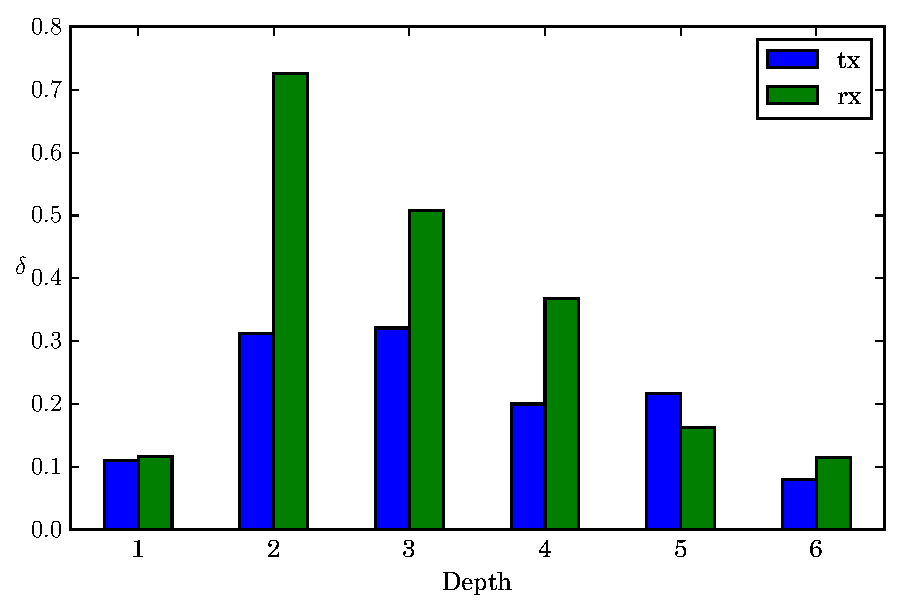
\includegraphics[width=0.5\textwidth]{figures/global_route.pdf}}
    \caption{$\delta$ par profondeur}
    \end{figure}

  \pnote{
    - Remarque de Nathalie: On néglige les ACK. Notre modèle est perfectible.
    Cependant les ack prennent peu de temps à transmettre et ne suffirai probablement pas à rattraper le retard.
  }

\end{frame}

\begin{frame}{Mesure active périodique}
  \begin{block}{Objectifs}
    \begin{itemize}
      \item Apprendre le biais de l'estimation passive
    \end{itemize}
  \end{block}
  \begin{alertblock}{Modèle correctif}
    \begin{align}
      \widehat{X}(t) &= X(t_r) + \epsilon(t_r)\frac{t - t_r}{T}\\
      \epsilon(t_r) &= \alpha (X(t_r) - \widehat{X}(t_r)) + (1 - \alpha)\epsilon(t_{r-1})
      \label{supervision:eqn:bias}
    \end{align}
  \end{alertblock}
  \begin{block}{Topologie expérimentale}
    \begin{itemize}
      \item 21 nœuds
      \item $\alpha = 0.25$
      \item Mesure active toutes les 25 secondes
    \end{itemize}
  \end{block}
  \pnote{
    Meme condition de trafic - Cooja/powertracker - 200 secondes
  }
  \pnote{
    alpha faible va privilégier les tendances de fond
  }
\end{frame}

\begin{frame}\frametitle{Évolution de l'erreur d'estimation}
  \begin{figure}[ht]
    \centering
    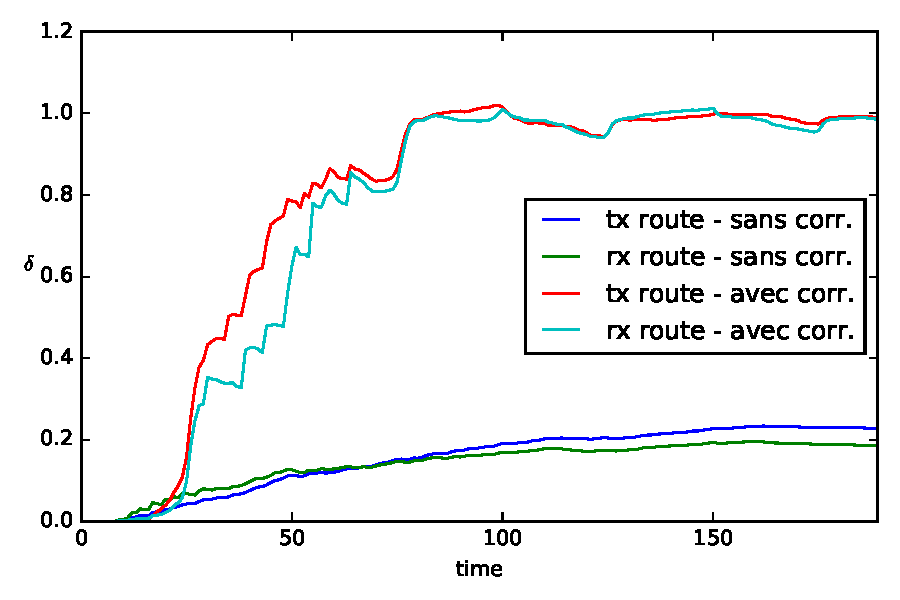
\includegraphics[width=\textwidth]{figures/mesure_active.pdf}
  \end{figure}
\end{frame}


\begin{frame}\frametitle{Conclusion}

  \begin{block}{Supervision}
      \begin{itemize}
        \item La connaissance de la topologie améliore la précision
        \item Calibration par strobing validée mais insuffisante
        \item Recalibrations nécessaires pour cette configuration
      \end{itemize}
  \end{block}

  \begin{block}{Ouvertures}
    \begin{itemize}
      \item Couche MAC plus fiable et déterministe (TSCH)
      \item Différentes topologies
    \end{itemize}
  \end{block}

  \pnote{
    - La supervision passive bien qu'imprécise fournit une quantité minimale d'information
  }
  \pnote{
    - La fiabilité des couches basses est essentielle pour construire des modèles fiables
  }

\end{frame}

\begin{frame}{Publication}
    Rémy Léone, Jérémie Leguay, Paolo Medagliani, Claude Chaudet.
    \newblock {Tee: Traffic-based energy estimators for duty-cycled Wireless Sensor Networks}.
    \newblock {\em {IEEE International Conference on Communication (ICC)}}, page~6749-6754, Londres, 2015.
\end{frame}
